\chapter{Agent Harnesses: Control Flow, Isolation, and Durable Effects}\label{ch:C20}
Harness$^2$ and RRSI make a current experimental boundary explicit: a frozen backbone can be surrounded by a changing execution procedure, and the resulting gains belong to the configured system rather than automatically to the checkpoint~\cite{corpus261014224,rrsi2026}. Harness$^2$ adds inference and model-based selection whose cost and evaluator dependence matter; RRSI limits repeated selection against a finite evolve set. These 2026 cases motivate the central question here: which state transitions changed, what evidence selected them, and can the claimed benefit survive independent tasks and runtime failures?

A model supplies a conditional distribution over candidate actions. A harness decides which observations enter that conditional distribution, which candidates become executable operations, how their effects are recorded, and what happens when execution stops unexpectedly. Consequently, harness behavior changes the effective policy even when model parameters remain fixed. An evaluation that reports only a model identifier omits part of the system being evaluated. Conversely, an improved harness does not demonstrate that the underlying model learned a new capability.

The engineering objective is controlled progress under incomplete observations and partial failures. Reliability requires separating three claims: the agent selected a sensible action, the runtime executed the intended operation, and the operation produced a state satisfying the task. A successful transport response proves none of the other two. This chapter derives an execution contract, examines its failure windows, and connects implementation choices to experiments. The discussion extends the state-consistency analysis of Chapter~\ref{ch:C17} and the interface constraints of Chapter~\ref{ch:C18}.

\section{The effective policy includes the harness}\label{sec:C20:policy}
Let $H_t$ denote the recorded interaction history, $C_t$ the constructed model context, $M_t$ persistent memory, and $E_t$ environment state. A harness configuration $h$ includes a context constructor $g_h$, action parser $p_h$, scheduler, authorization checks, and stopping policy. Let $S_t$ be the recorded execution state, defined in the next section. Let $\mathcal Z$ be the countable set of stopped output records and $\mathcal A$ the dispatch-action space augmented with a no-effect rejection outcome. Assume termination for this single-call model; otherwise nontermination needs its own mass as in Chapter~\ref{ch:C02}. For $z_t\in\mathcal Z$ and $a_t\in\mathcal A$, the induced distribution is
\begin{equation}
 \overline\Pi_{\theta,\delta,h}(a_t\mid S_t)=\sum_{z\in\mathcal Z}
 Q_{\theta,\delta}(z\mid C_t)
 K_h(a_t\mid p_h(z),S_t;\alpha_t).
\end{equation}
Here $Q_{\theta,\delta}$ is the normalized stopped law of the actual decoder, $C_t=g_h(S_t)$ uses only the declared policy-visible projection, and $K_h$ is the parser/enforcement kernel under current authority epoch $\alpha_t$. Its output is a dispatched action or a no-effect outcome; dispatch is not remote commitment. It can reject malformed output or substitute a deterministic fallback. A request for model repair is instead a transition to another inference call, not a free operation inside this single-call expression. Its likelihood, latency and cost belong to the subsequent trajectory. This distinction prevents a repair-enabled harness from being analyzed as though it executed only the final valid response. A parser that silently normalizes an ambiguous filename makes a policy decision; it is not merely formatting infrastructure.

This decomposition explains why two products using the same checkpoint can differ substantially. They may expose different tools, truncate different observations, retry at different boundaries, or terminate after different evidence. The code-as-harness survey organizes these mechanisms through interfaces, execution feedback, memory, and coordination~\cite{corpus260518747}. Its taxonomy is useful architectural synthesis, but does not establish that every additional mechanism improves performance. Additional machinery can increase failure opportunities and conceal the origin of a gain.

A clean causal comparison specifies the treatment as a configuration change. Suppose the treatment adds a planning file and a summarization tool. Its measured effect combines extra inference, altered context, persistent state, and a new action interface. Attributing the result to ``planning'' requires controls that preserve the other differences. One control allocates the same additional model calls to independent attempts; another retains the file interface but disables learned updates; a third supplies an oracle summary to estimate headroom. None is sufficient alone because the treatment can interact with task length and tool latency.

Harness adaptation creates a second policy. RRSI searches over harness changes while holding backbone weights fixed and constrains proposal and selection behavior~\cite{rrsi2026}. The important lesson is not a universal numerical gain, but that repeated selection against a finite evolve set can optimize quirks rather than transferable procedures. A runtime should therefore record the complete harness identity alongside the model and memory version. Reconstructing a trajectory with a later parser or prompt can change its interpretation even when every raw message is preserved.

For implementation, define the smallest state transition with an externally meaningful outcome. Avoid making an entire conversational turn the only transaction boundary: it can contain multiple tool effects and multiple opportunities for interruption. Also avoid recording every generated token as a committed action. Token streams are provisional inference products; an executable operation begins only after parsing, authorization, and allocation of a stable identity.


\section{Execution state and semantic commitments}\label{sec:C20:state}
An execution record needs more than messages. A useful state is
\begin{equation}
 S_t=(H_t,C_t,M_t,J_t,A_t,V_t,B_t),
\end{equation}
where $J_t$ is an operation journal, $A_t$ authorization state, $V_t$ the compatibility tuple, and $B_t$ the remaining budget. The environment is observed through versioned evidence rather than assumed to be fully contained in $S_t$. An email service, remote repository, or browser session can change independently. Storing an observation is not locking the corresponding external object.

The journal distinguishes intent, dispatch, observation, and reconciliation. An intent says what the application authorized. Dispatch records that a request crossed a boundary. Observation records the response or the absence of one. Reconciliation establishes what external state now exists. These states must remain distinct because a timeout after dispatch is observational uncertainty, not proof of failure. Retrying an uncertain operation without examining its effect can duplicate it.

Three invariants make this distinction operational. First, every effectful request refers to an authorized intent whose argument hash and policy epoch match the request. Second, every committed result identifies the exact intent and the evidence used to accept it. Third, resumption does not infer completion from an optimistic natural-language summary. It consults the journal and, when necessary, the authoritative service. A summary may help the model reason about the result, but it cannot replace the result record.

Typed states also prevent a subtle category error: task completion and runtime completion are different predicates. Let $T(S)$ mean the user task is satisfied, $Q(S)$ mean required checks passed, and $R(S)$ mean no operation remains unresolved. A defensible terminal condition is $T(S)\land Q(S)\land R(S)$ under the declared specification. A model-generated ``done'' token establishes only that the inference process proposed termination. A quality gate may still misclassify the output, so even this terminal condition is relative to the validators' coverage.

Application frameworks expose parts of these distinctions. The inspected LangGraph persistence documentation separates thread checkpoints from cross-thread stores~\cite{langgraph2026docs}. That distinction should not be collapsed into a claim that a checkpoint already implements semantic memory. Checkpoints support restoration of declared graph state. Cross-thread stores retain application records. Neither feature independently establishes truth, relevance, authorization, or successful external-effect recovery.

The practical design choice is to make semantic commitments inspectable. A tool receipt should include object identifiers, version or timestamp, effective principal, argument digest, and verification status. Where a remote service exposes no stable receipt, record that limitation explicitly. It may justify requiring review before a consequential retry. The runtime must not manufacture transactional guarantees that the connected service does not provide.


\section{Crash consistency and uncertain effects}\label{sec:C20:crashes}
Consider a request to create an external issue. A crash can occur before intent persistence, after persistence but before dispatch, after remote creation but before response receipt, or after receipt but before local commitment. These windows require different recovery actions. Before dispatch, replay can safely issue the request. After uncertain dispatch, recovery must first determine whether the remote creation occurred. After a committed receipt, replay should return the recorded outcome rather than create a second object.

An idempotency key helps only if the remote service gives it the required semantics. Reusing an application-generated string does not by itself make an API idempotent. The service must scope the key appropriately, retain its association long enough, reject incompatible reuse, and return a stable result. A short retention period can make an old replay unsafe. Idempotency may also apply only to one endpoint, leaving downstream notifications or billing outside the guarantee.

An execution protocol can be specified as a branch-dependent state transition. Let $i$ be the intent, $J$ the journal in $S$, $\alpha$ current authority, and $\nu$ the recorded release version. Define $v(i)\in\{0,1\}$ by intent-schema validation. Let $a_J(i,J,\alpha)$ govern access to the corresponding journal records and $a_D(i,\alpha)$ govern new external dispatch. Read access to a historical receipt is distinct from permission to repeat its effect; either denied check produces its own non-effect outcome. For a valid intent, $k=\eta(i)$ is its stable logical-operation identifier. The lookup $\sigma_J(k)\in\{0,1,2,3\}$ distinguishes absence, persisted intent, marked dispatch without a terminal verdict, and committed terminal verdict. Define $\gamma(i,S)=1$ exactly when $v(i)=1$, $a_J(i,J,\alpha)=1$, and either $\sigma_J(k)=0$ or the recorded logical intent identity and exact payload match $i$; otherwise $\gamma(i,S)=0$. This binding and record-access check precedes replay and reconciliation as well as fresh dispatch; revoking write authority need not revoke legitimate access to a past receipt. For a recorded operation, $\rho_J(k)$ returns its recorded outcome, or $\upsilon$ when terminal evidence remains unresolved. The top-level transition is
\begin{equation}
 \Phi(i,S)=
 \begin{cases}
  (J,\bot),&\gamma(i,S)=0,\\
  (J,\rho_J(k)),&\gamma(i,S)=1,\ \sigma_J(k)=3,\\
  \Phi_R(i,S;k),&\gamma(i,S)=1,\ \sigma_J(k)=2,\\
  \Phi_0(i,S;k),&\gamma(i,S)=1,\ \sigma_J(k)\in\{0,1\}.
 \end{cases}
\label{eq:C20:execution_branches}
\end{equation}
For $a_D(i,\alpha)=0$, $\Phi_0(i,S;k)=(J,\bot_A)$ without dispatch. Otherwise the following fresh-dispatch equations describe the acknowledged-write branch:
\begin{equation}
\begin{aligned}
 J_1&=\mathcal I(J;k,i,\nu),\\
 J_2&=\mathcal D(J_1;k),\\
 o&\sim\mathcal T(\,\cdot\mid i,k),\qquad J_2\ne\bot_J,\\
 J_3&=\mathcal O(J_2;k,o),\qquad g=\mathcal V(i,o),\\
 J_4&=\mathcal C(J_3;k,o,g),\\
 \Phi_0(i,S;k)&=(J_4,\rho_{J_4}(k)).
\end{aligned}
\label{eq:C20:fresh_dispatch_transition}
\end{equation}
Each journal operator returns an acknowledged journal or $\bot_J$; the next line is evaluated only on an acknowledged branch. Branch selection and the dispatch-marker transition require a serialized dispatcher per key or an equivalent atomic, fenced claim. A read followed by unconditional writes is insufficient under concurrent recovery. A storage failure returns the last acknowledged journal and a storage-error outcome, without inventing a new external status. In particular, intent or dispatch-marker failure prevents a new call, whereas receipt-write failure after a call can require reconciliation. Here $\mathcal I$ persists the versioned intent, $\mathcal D$ durably marks dispatch, $\mathcal T$ invokes the external tool under key $k$, $\mathcal O$ persists the returned observation, and $\mathcal V$ evaluates the effect evidence. The operator $\mathcal C$ persists its verdict $g\in\{-1,0,1\}$, denoting negative, unresolved, and positive. Only a terminal verdict justified by adequate evidence yields $\sigma=3$; $g=0$ preserves $\sigma=2$ and $\rho=\upsilon$. An unresolved first-call result therefore remains explicitly unresolved rather than acquiring certainty from the name of a commit routine. Reuse of an existing intent requires equality of its payload and declared identity; a key collision cannot authorize substitution.

For a previously marked dispatch, let $\widehat o=\mathcal R(i,J;k)$ denote evidence obtained by an independently authorized status/reconciliation operation, with $\upsilon$ denoting an unresolved observation. If no permitted reconciliation path exists, $\mathcal R$ returns $\upsilon$ without issuing a query. Define
\begin{equation}
\begin{aligned}
 \widehat J&=\mathcal C\bigl(J;k,\widehat o,
                         \mathcal V(i,\widehat o)\bigr),\\
 \Phi_R(i,S;k)&=
 \begin{cases}
  (J,\upsilon),&\widehat o=\upsilon,\\
  (J,\bot_J),&\widehat o\ne\upsilon,\ \widehat J=\bot_J,\\
  (\widehat J,\rho_{\widehat J}(k)),&\widehat o\ne\upsilon,\ \widehat J\ne\bot_J.
 \end{cases}
\end{aligned}
\label{eq:C20:reconciliation_transition}
\end{equation}
The definition of $\widehat J$ is evaluated only when $\widehat o\ne\upsilon$; a failed reconciliation write returns the last acknowledged journal and a storage error rather than applying a lookup to $\bot_J$. Neither the unknown branch nor replay of a terminal record invokes $\mathcal T$. The journal-access policy is checked before branch selection; a reconciliation query needs its own applicable permission. New dispatch always checks current effect authority under the remote service's concurrency contract. Neither reading a receipt nor reconciling status grants permission to repeat the original write. These relations specify required ordering and evidence semantics; they do not prove that a particular runtime or remote service implements them.
Persisting a dispatch marker before calling introduces a conservative ambiguity: the marker may exist even if the request never left the process. Marking it after the call introduces the opposite ambiguity: an effect can exist without a marker. No local ordering removes both without cooperation from the remote system. This is the fundamental reason a journal cannot alone provide exactly-once external effects.

Compensation is a separate operation. Closing an erroneously created issue does not erase notifications already sent. Reverting a file does not retract information copied by another process. A compensating operation can restore an application invariant while leaving residual effects. Therefore recovery reports should distinguish restored local state, reconciled external state, and irrecoverable consequences. This classification supports meaningful incident analysis and prevents rollback metrics from becoming cosmetic.

Fault-injection experiments should target these exact windows. Kill the worker after remote acceptance but before local receipt persistence; interrupt between verification and commit; corrupt one journal entry; delay a response beyond the retry threshold. Compare stateless retry, checkpoint replay, and journal-based reconciliation under identical fixtures. Measure duplicate effects, unresolved operations, recovery latency, and task completion. These are proposed experiments; no failure rate is inferred from the protocol's appearance.


\section{Context construction is runtime scheduling}\label{sec:C20:context}
Context management determines which parts of execution state the policy can use. A journal may be complete while $C_t$ omits the operation that explains a pending effect. Conversely, a summary may assert completion that the journal never committed. The harness therefore needs a projection contract between authoritative state and model-visible state. For a projection claiming effect-aware planning, the relevant unresolved operations and active constraints need a usable representation. Exact authority and sensitive effect evidence can remain privileged, with a policy-safe status projection; copying every grant or credential into the prompt is unnecessary.

A projection can be tested against invariants without requiring an exact semantic equivalence oracle. For example, inject a pending-operation record and verify that the constructed context includes its stable identifier and uncertainty state. Insert a revoked capability and check that the tool registry removes it regardless of whether the model remembers an earlier grant. These checks establish structural properties. Whether a compressed explanation preserves every decision-relevant fact remains a behavioral question and requires task-level evaluation.

Agentic Context Management supplies model-directed offloading and retrieval mechanisms~\cite{corpus260723809}. Its live-run raw mirror can preserve access to discarded content, but archival retention does not guarantee that the agent retrieves the right item at the right time. Its reported benefits also depend on a capable backbone and reimplemented baselines. This distinction matters for runtime design: storing raw history is a recovery affordance; selecting useful context is an additional policy with cost, latency, and failure modes. The snapshot-only restore path discussed in Chapter~\ref{ch:C13} does not preserve a previously separate raw archive by itself~\cite{repo_acm2026}.

An execution scheduler can reserve a protected context region for authoritative status and separately allocate a discretionary region for retrieved evidence. Protection should mean application-controlled serialization, not merely an instruction asking the model to respect a textual heading. The trusted region should be generated from current state on every call. If a retrieved document can overwrite it through string concatenation or malformed role boundaries, the separation is nominal rather than enforced.

The resource constraint couples context and scheduling. Long tool outputs increase prefill cost and may delay other sessions. An aggressive truncation policy improves throughput but can remove the evidence needed for reconciliation. A token budget should therefore distinguish required status tokens, candidate evidence tokens, and speculative reasoning allocations. When the budget cannot accommodate required state, the runtime should reduce work, retrieve narrower evidence, or request a bounded continuation. Silent removal of constraints is not a legitimate optimization.

Evaluate these choices with task-length and output-size strata. Average success can hide a regime where compaction helps short tasks but fails after the first interruption. Include a baseline that keeps authoritative status fixed while varying only discretionary history. This separates failures of the projection contract from failures of the model to interpret otherwise available evidence. Report the cost of reconstructing omitted evidence, not only the reduction in visible prompt length.


\section{Budgets cancellation and backpressure}\label{sec:C20:budgets}
A runtime executes under several budgets that are not interchangeable. Tokens constrain inference volume; wall-clock deadlines constrain responsiveness; tool quotas constrain access; monetary limits combine model and service costs; risk budgets constrain permitted effects. Converting all of them into one scalar can obscure hard requirements. A cheap operation may still be unauthorized, and a low-token plan may wait indefinitely on a remote tool.

Represent remaining resources by a vector $B_t$ and each candidate action by a distribution of costs. Admission requires hard constraints to hold before expected utility is considered. For a deadline $D\geq0$, current elapsed time $t\in[0,D]$, nonnegative uncertain duration $L(a)$, and tolerated miss probability $\epsilon\in(0,1)$, a chance constraint $\Pr(L(a)\leq D-t)\geq1-\epsilon$ is meaningful only when the duration model is calibrated for the workload. A mean-latency estimate does not establish a tail guarantee. Timeouts truncate observations and can bias the estimated distribution if treated as ordinary successful durations.

A hard budget also needs reservations under concurrency. For a scalar budget $B_0$, let $s_t$ be settled spend, $P_t$ outstanding operations and $r_i$ the reserved upper cost of operation $i$. Require
\begin{equation}
 s_t+\sum_{i\in P_t}r_i\leq B_0.
\end{equation}
Admission checks the invariant and reserves $r_i$ before dispatch in one linearizable budget-ledger transition. Settlement must use the same ledger and atomically add $c_i$ to settled spend while removing $r_i$ from outstanding reservations, with $0\leq c_i\leq r_i$. It is idempotent under the logical-operation key: a repeated settlement returns the recorded result without charging or releasing again. Admission, settlement and release share one serialization order. Releasing a reservation before recording its charge would let another admission consume the apparent balance and invalidate the bound. Under these assumptions, each ledger transition preserves the invariant by induction. Vector budgets use componentwise inequalities. This guarantee requires valid cost bounds and linearizable, crash-consistent accounting; an expected-cost estimate or atomic reservation alone is insufficient. Cancellation does not release a reservation until the remaining charge or effect is bounded. An unbounded remote billing path cannot be turned into a hard cap by local accounting alone.

Cancellation propagates through an ownership tree. A parent may cancel its own inference yet leave a remote command, browser navigation, or delegated worker running. The runtime needs a record of outstanding operations, cancellation support for each tool, and a reconciliation strategy for tools that cannot stop. Returning control to the user does not prove that background effects have ceased. This distinction is particularly important when a later instruction changes authorization while an earlier operation remains in flight.

Backpressure prevents an overloaded system from amplifying its own failures. If a tool slows down, retries can increase offered load and make recovery less likely. A retry policy should distinguish transport failure, rate limiting, invalid arguments, and uncertain completion. Backoff addresses congestion; it does not repair a malformed request. A circuit breaker prevents repeated calls to a failing dependency but must preserve evidence about abandoned work. Otherwise the agent may reinterpret a dependency outage as evidence that a fact or object does not exist.

The scheduling objective must also include fairness. A single long-running agent can occupy scarce browser sessions or large KV allocations while shorter requests wait. Preemption can improve fairness but increases checkpoint and reconstruction cost. The appropriate policy depends on whether progress is checkpointable and whether external operations can be safely suspended. A runtime should expose these workload properties rather than apply one universal quantum to every tool.

Benchmark admission and cancellation under open-loop arrival processes, not only fixed concurrency. Fixed concurrency reduces offered load when latency rises and can conceal instability. Report queueing delay separately from execution time, and include rejected or cancelled work in the relevant denominator. Tail latency, budget overshoot, orphaned operations, and completed useful work collectively describe whether the scheduler preserves service objectives under stress.



Figure~\ref{fig:C20:overview} isolates the mechanism and its stated information boundaries.
\begin{figure}[!htbp]
\centering
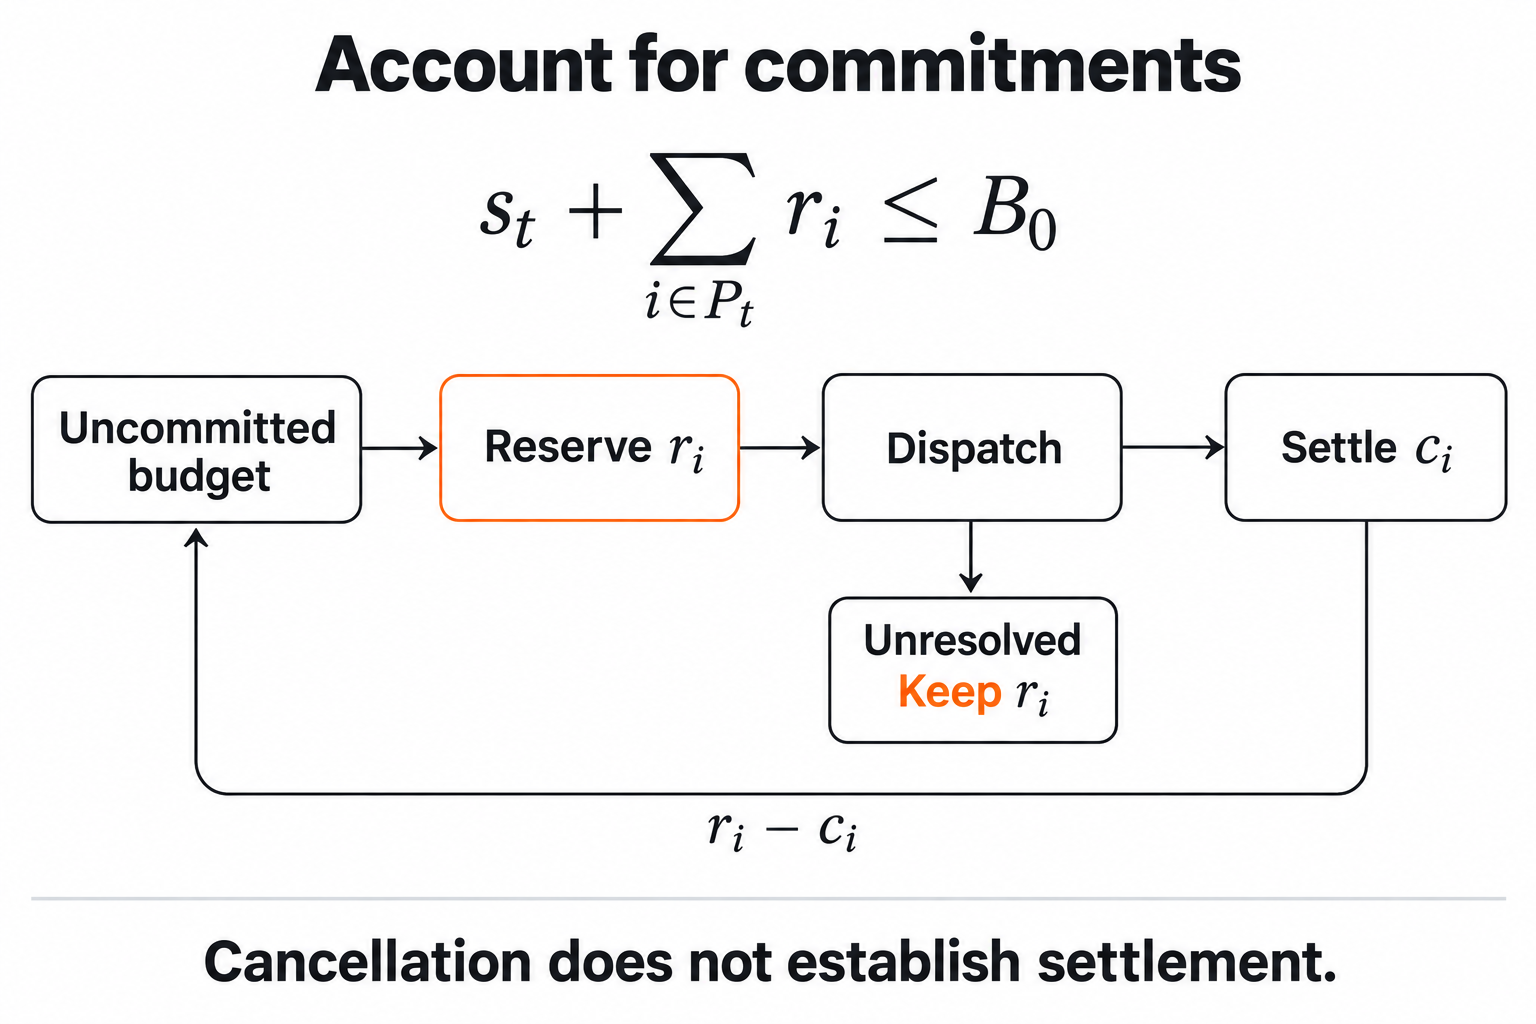
\includegraphics[width=\linewidth]{book/figures/assets/F20review.png}
\caption{A hard-budget invariant accounts for settled spend and bounded outstanding commitments. Admission reserves an upper cost before dispatch. Keyed idempotent settlement atomically records the actual charge and releases only the unused reservation in the same linearizable ledger used for admission. Unresolved operations retain commitments until remaining charges are bounded; cancellation alone does not release them.}
\label{fig:C20:overview}
\end{figure}

\section{Implementation boundaries and evidence}\label{sec:C20:implementation}
An inspectable harness exposes action parsing, context construction, tool dispatch, state persistence, stopping, and error recovery as separable modules. Code location alone is insufficient: a module can delegate essential behavior to a proprietary endpoint. The implementation record should identify the local revision, external service version where available, configuration, and which semantics remain opaque. This is the minimum needed to connect an algorithm to an identifiable execution path.

The OpenAI Agents SDK documentation describes an application-owned deployment path, whereas a managed agent service supplies a different runtime boundary~\cite{openai2026agents}. A thin SDK wrapper does not transfer ownership of application storage, tool semantics, or approvals to the provider. Conversely, a hosted runtime may maintain session state without exposing the underlying scheduler. These are role differences, not evidence that one architecture is universally more reliable. Chapter~\ref{ch:C22} compares their consequences without importing product priority rankings.

Harness\textsuperscript{2} illustrates adaptation of execution and improvement harnesses using behavioral comparisons and experience reuse~\cite{corpus261014224}. Without ground-truth task verifiers, such feedback remains vulnerable to shared model biases and execution variance. More editor sessions can improve the search over changes while also increasing cost and selection opportunities. A runtime supporting this mechanism needs candidate isolation, a record of rejected changes, and a rollback boundary that includes prompts, tools, and memory interpretation.

The current Harness\textsuperscript{2} source distinguishes logical stage accounting from all invocation costs. Its \path{core/ledger.py} checks rollout and improvement-stage identities $R=4k$ and $P=3k$ for recursion budget $k$, rejects duplicate stage labels, and separately records retry attempts. Selection and reflection are outside this ledger's stated counting boundary~\cite{cumb2026harness2code}. These are source-level count identities, not measurements of runtime or total expense. A complete cost comparison must join those stages with selection, reflection and failed invocations. The ledger is an adaptation-budget record, not a transactional journal proving remote-effect recovery.

An implementation audit should begin with one complete request, not an abstract class diagram. Trace the request from input serialization to terminal artifact, identify every mutable dependency, and enumerate where errors are caught or suppressed. A broad exception handler that returns a plausible textual tool result can turn infrastructure failure into misleading model evidence. A successful deserialization test will not expose that defect; an injected dependency outage will.

The strongest verification combines local contract checks with end-to-end behavioral experiments. Contract tests can establish that duplicate operation identifiers are rejected or that schema changes invalidate cached decisions. They cannot establish that a proposed patch satisfies an underspecified user task. Behavioral tests can estimate task reliability but may miss rare transactional windows. The two forms of evidence answer different questions and should remain separately reported.

The practical implication is a narrow but consequential design principle: authoritative execution state should be machine-checkable, recoverable, and distinct from model narration. The model remains essential for interpreting uncertain tasks and choosing useful actions. The runtime supplies the boundaries within which those choices can be evaluated and acted upon. Reliability emerges from their interaction; neither a fluent agent nor a durable database independently establishes it.

\section{A worked analysis of a recoverable repository workflow}\label{sec:C20:case}
Consider a repository-maintenance agent asked to update a dependency, run tests, and prepare a reviewable change. Its environment has four independently mutable surfaces: the checkout, dependency registry, test infrastructure, and remote review service. The task is deliberately narrower than autonomous deployment. The relevant success predicate requires the intended version change, passing required tests under the declared environment, and a review artifact referring to the verified revision. A passing local command is not sufficient if the remote artifact contains another commit.

Start by assigning an immutable task identifier and recording the initial repository commit. The package resolution step produces a lockfile whose content depends on registry state as well as the requested version. Therefore the transition record must include the resolved artifact identity, not only the human-readable version string. A registry can republish metadata or a moving tag can resolve differently. Replaying the same command later may produce different bytes even when the agent's prompt is unchanged. Reproducibility requires controlling this dependency or recording that it remains uncontrolled.

Next, the agent edits files in a workspace branch. The harness can checkpoint a filesystem snapshot before execution, but the snapshot does not capture every external dependency. A test can consult network services, local caches, or environment variables. The verification record should bind the resulting verdict to the workspace digest, test selection, dependency manifest, and relevant environment identity. If the model changes a source file after tests finish, the prior verdict becomes stale. The runtime can enforce this mechanically by invalidating verdicts whose dependency digests no longer match the current artifact.

This binding can be expressed as an acceptance rule. Let $x$ be the proposed artifact, $d(x)$ its digest, $v$ a verifier configuration, and $r$ a recorded test outcome. The gate accepts only if $r$ was produced for $(d(x),v)$ and the required checks passed. The rule establishes correspondence between artifact and evidence; it does not establish completeness of the tests. An independent specification defect remains possible. The separation is useful because it prevents a simple engineering mismatch from being obscured by philosophical uncertainty about correctness.

Now introduce a crash after the remote review service creates the artifact but before the harness stores its identifier. Replaying the create request can produce duplicates. If the service supports an idempotency key, recovery uses the original key. If it does not, the agent can query for an artifact marked with the task identifier and expected commit digest. That query may return zero, one, or several matches. Zero results are not conclusive under eventual consistency. Several results require reconciliation rather than arbitrary selection. A bounded waiting policy and an unresolved status are more accurate than asserting that the operation failed.

The cost of naive retries can be analyzed without inventing a measurement. Conditional on one dispatch, let $A$ be the event that the request takes effect but its acknowledgment is lost, and let $R$ mean recovery retries without reconciliation. For $q=\Pr(A)>0$ and $r=\Pr(R\mid A)$, the chain rule gives $\Pr(A\cap R)=qr$. No independence assumption is needed with this conditional definition of $r$. If $q=0$, the joint event has probability zero without defining $r$. Under the one-retry model this is a duplicate opportunity. The actual duplicate probability also depends on remote deduplication and whether the operation is intrinsically idempotent. This expression is not an estimate of any product. It identifies two distinct intervention targets: reduce acknowledgment ambiguity or eliminate blind retries. Improving model reasoning alone need not reduce either one.

Suppose authorization changes while the task is interrupted. The original grant allowed preparation of a review artifact, but the operator later revokes remote write access. Restoring the old checkpoint must not restore the old grant as if it were still current. Recovery loads execution progress from the checkpoint and authorization from the authoritative policy service. The resumed model may still see a historical permission statement in $H_t$; the tool boundary must reject a newly attempted write under the current epoch. This example shows why replay fidelity and present authorization can legitimately diverge.

Deletion introduces another dependency. If a user requests removal of sensitive task material, deleting the current context does not remove journal payloads, filesystem checkpoints, test logs, remote artifacts, or indexing copies. A retention service needs a dependency inventory and a distinction between records required for audit and content permitted for reuse. Where legal or operational retention prevents immediate physical deletion, the system should record the constraint and prevent subsequent model retrieval. It should not describe a tombstone as completed physical erasure. Chapter~\ref{ch:C29} examines the authority and governance implications.

A controlled evaluation of this workflow uses deterministic repository fixtures and instrumented remote-service simulators. Each fixture specifies the allowed edits, required checks, and permitted remote effects. Failures are injected at journal, network, verifier, and artifact-publication boundaries. The primary unit is a task instance with its complete failure schedule, not an individual model call. Paired schedules allow comparison of recovery strategies without confounding one strategy with easier failures. Model sampling remains a separate repeated-run factor, and uncertainty should preserve clustering by fixture.

Report artifact correctness, stale-verdict acceptance, duplicate creations, authorization violations, unresolved outcomes, and complete execution cost. A runtime can achieve fewer duplicates by refusing all remote work, so benign completion must be reported alongside containment. It can achieve low mean latency by abandoning difficult recoveries, so abandoned and timed-out runs remain visible. These paired metrics force the experiment to evaluate the desired tradeoff rather than reward a degenerate implementation. The worked example yields no universal winner, but it supplies a precise testable distinction between durable progress and merely persistent conversation.

